\documentclass[11pt,a4paper]{article}
\usepackage[utf8]{inputenc}
\usepackage[english]{babel}
\usepackage{amsmath}
\usepackage{amsfonts}
\usepackage{amssymb}
\usepackage{graphicx}
\usepackage{kbordermatrix}
\usepackage{listings}
\usepackage{multicol}
\usepackage{graphicx}
\setlength{\columnsep}{2cm}

\lstdefinestyle{mystyle}{
    breakatwhitespace=false,         
    breaklines=true,                 
    captionpos=b,                    
    keepspaces=true,                 
    numbers=left,                    
    numbersep=15pt,                  
    showspaces=false,                
    showstringspaces=false,
    showtabs=false,                  
    tabsize=2
}
\lstset{style=mystyle}


\newenvironment{Figure}
  {\par\medskip\noindent\minipage{\linewidth}}
  {\endminipage\par\medskip}

\usepackage[left=2cm,right=2cm,top=2cm,bottom=2cm]{geometry}
\author{UUN: S1796157}
\title{Algorithmic Game Theory and Applications (INFR11020) Coursework 1}
\date{}
\begin{document}
\maketitle
\section{Question 1}
First of all, we can easily find two Nash Equilibria by analyzing the best
responses for each player to the strategy of the other player. We are sure
that they are NE since each of the players cannot get a better payoff by
deviating from its strategy. Therefore, the first two \textit{pure} NEs are:
\[
\{(1,0,0,0) \quad (0,1,0,0)\} \quad \hbox{and} \quad \{(0,0,1,0) \quad (0,0,1,0)\}
\]
We now start looking for other possible \textit{mixed} NEs. We use the iterated strictly
dominant strategy (ISDS) by removing from the game $G$ all the \textit{pure strictly dominated}
strategies and all the \textit{mixed strictly dominated strategy}. We can easily notice
from the payoff matrix that there are no pure SDS, so we start looking for mixed SDS:
\begin{align*}
&\kbordermatrix{
& A' & B' & C' & D'\\
A & (7,4) & (7,6) & (4,4) & (4,3)\\
B & (9,5) & (5,3) & (4,6) & (8,4)\\
C & (9,4) & (5,3) & (5,8) & (5,4)\\
D & (6,8) & (5,9) & (4,8) & (9,8)
}
\xrightarrow{\frac{1}{3}A'+\frac{1}{3}B'+\frac{1}{3}C'>D'}
\kbordermatrix{
& A' & B' & C'\\
A&(7,4) & (7,6) & (4,4)\\
B&(9,5) & (5,3) & (4,6)\\
C&(9,4) & (5,3) & (5,8)\\
D&(6,8) & (5,9) & (4,8)
}
\\
&\xrightarrow{\frac{1}{3}A+\frac{1}{3}B+\frac{1}{3}C>D}
\kbordermatrix{
& A' & B' & C'\\
A&(7,4) & (7,6) & (4,4)\\
B&(9,5) & (5,3) & (4,6)\\
C&(9,4) & (5,3) & (5,8)
}
\xrightarrow{\frac{3}{4}B'+\frac{1}{4}C'>A'}
\kbordermatrix{
& B' & C' \\
A&(7,6) & (4,4)\\
B&(5,3) & (4,6)\\
C&(5,3) & (5,8)
}
\\
&\xrightarrow{\frac{1}{2}A+\frac{1}{2}C>B}
\kbordermatrix{
& B' & C' \\
A&(7,6) & (4,4)\\
C&(5,3) & (5,8)
}
\end{align*}
We have now a \textit{reduced} payoff matrix $M'$, which is equivalent to the original one $M$
(from here we can clearly see the previous \textit{pure} NE). To find the remaining \textit{mixed}
strategies we know that from the Corollary of Nash's Theorem, if the row player is playing
against a mixed strategy of the column player, then the strategies of the row player must be
the best response to the strategies of the column player (the same applies also for the
column player with respect to the row player).
\medskip

We assign probabilities to the strategies of both players:
\begin{equation*}
\kbordermatrix{
& q & (1-q)\cr
p& (7,6) & (4,4)\cr
(1-p) & (5,3) & (5,8)}
\end{equation*}

\begin{equation*}
7q+4(1-q)=5q+5(1-q) \qquad 6p+3(1-p) = 4p+8(1-p)
\end{equation*}
If we solve the previous equations we will get $p=\frac{5}{7}$ and $q=\frac{1}{3}$. Therefore, since the
\textit{reduced} payoff matrix is equal to the original payoff matrix, we can derive the last NE:
\begin{equation*}
\{ (\frac{5}{7}, 0,\frac{2}{7}, 0, 0), (0, \frac{1}{3}, \frac{2}{3}, 0)\}
\end{equation*}
In conclusion, the NEs for this game are:
\begin{gather*}
\{(1,0,0,0) \quad (0,1,0,0)\}\\
\{(0,0,1,0) \quad (0,0,1,0)\}\\
\{ (\frac{5}{7}, 0,\frac{2}{7}, 0, 0) \quad (0, \frac{1}{3}, \frac{2}{3}, 0)\}
\end{gather*}
By eliminating all the SD strategies we are sure to not have deleted any NE, since
SD strategies cannot be played with positive probability. Moreover, $p$ and $q$ were
uniquely determined, so there must exist only one \textit{mixed} NE. Therefore,
the NEs we found previously are the only NEs presents in this game $G$.

\section{Question 2}
Given the payoff matrix $A$ for player 1, we can build a linear program for solving Minmax
and get both the minmax value for this zero-sum game and the optimal strategy for player 1
($x^{T}=[x_1, x_2, x_3, x_4, x_5]$ represents the probability assigned to each strategy).
The LP associated to Player 1 is:
\begin{gather*}
\hbox{\textbf{Maximize}} \quad v\\
\hbox{\textbf{Subject to:}}\\
x^{T}A \geq v\\
x_1+x_2+\ldots+x_5 = 1\\
x_i \geq 0 \quad \forall \; i=1,\ldots,5
\end{gather*}
By maximizing $v$, we get $v=4.1862$ and the minmaximizer strategy for player 1, which
is equal to $(0.0994, 0.2793, 0.2017, 0.2736, 0.1460)$.
Regarding player 2, taking $y^T=[y_1,y_2,y_3,y_4,y_5]$ as the maxminimizer strategy, his LP becomes:
\begin{gather*}
\hbox{\textbf{Minimize}} \quad u\\
\hbox{\textbf{Subject to:}}\\
(-A)y \leq u\\
y_1+y_2+\ldots+y_5 = 1\\
y_i \geq 0 \quad \forall \; i=1,\ldots,5
\end{gather*}
By solving this problem, we get $u=4.1862$ and the maxminimizer strategy becomes equal to
$(0.3963, 0.1410, 0.3286, 0.0508, 0.832)$.
\medskip

It can be shown that the dual of the primal LP (the player 1's LP) is the same as
player 2's LP. This means that when solving the LP's dual problem we are
actually finding player 2's optimal strategy. That is the reason why $v=u$.
\newpage

\section{Question 3}

\subsection{a)}
We proceed as we did for the first exercise. From the Corollary of Nash's Theorem, if the row player is playing
against a mixed strategy of the column player, then the strategies of the row player must be
the best response to the strategies of the column player (the same applies also for the
column player with respect to the row player). Therefore, we assign probabilities to the strategies of both players:
\begin{equation*}
\kbordermatrix{
& x & y & 1-x-y \cr
p & (0,0) & (-1,1) & (1,-1) \cr
q & (1,-1) & (0,0) & (-1,1) \cr
1-p-q & (-1, 1) & (1,-1) & (0,0)
}
\end{equation*}
and then we solve the corresponding linear systems:
\begin{equation*}
\begin{cases}
q-(1-p-q) = -p +1 -p -q\\
-p +1 -p-q = p-q
\end{cases}
\qquad
\begin{cases}
x-(1-x-y) = -x +1 -x -y\\
-x +1 -x-y = x-y
\end{cases}
\end{equation*}
which lead to unique solutions $p=q=\frac{1}{3}$ and $x=y=\frac{1}{3}$. Therefore, the only NE in this
game is $\{(\frac{1}{3},\frac{1}{3},\frac{1}{3}),(\frac{1}{3},\frac{1}{3},\frac{1}{3})\}$ (since there 
are no pure NEs).

\subsection{b)}
\lstinputlisting[language=Python]{../exercise_3.py}
\newpage

The Python code presented is the one which was used to test the assumption that both of the
statistical mixed strategies converge to the unique NE. The program simulates many Rock-Paper-Scissor
sessions. Each of the players chooses its best response to the other player’s strategy by looking at the
strategy which maximizes its payoff (see the method on line 8). If we have multiple pure best responses,
the tie ruled used is to choose randomly one of them with uniform probability (line 18). After having
played many game sessions, we can clearly see how the statistical mixed strategy tend to converge to
the unique NE of the game. This is true regardless of which starting strategies players use (in the
code we can change the starting strategy by changing the contents of the dictionary on line 3). As a side note, in this program, we deal with the number of occurrences of rock/paper/scissors, without directly using probabilities, but this do not change the final outcome.
\begin{figure}[b!]
\centering
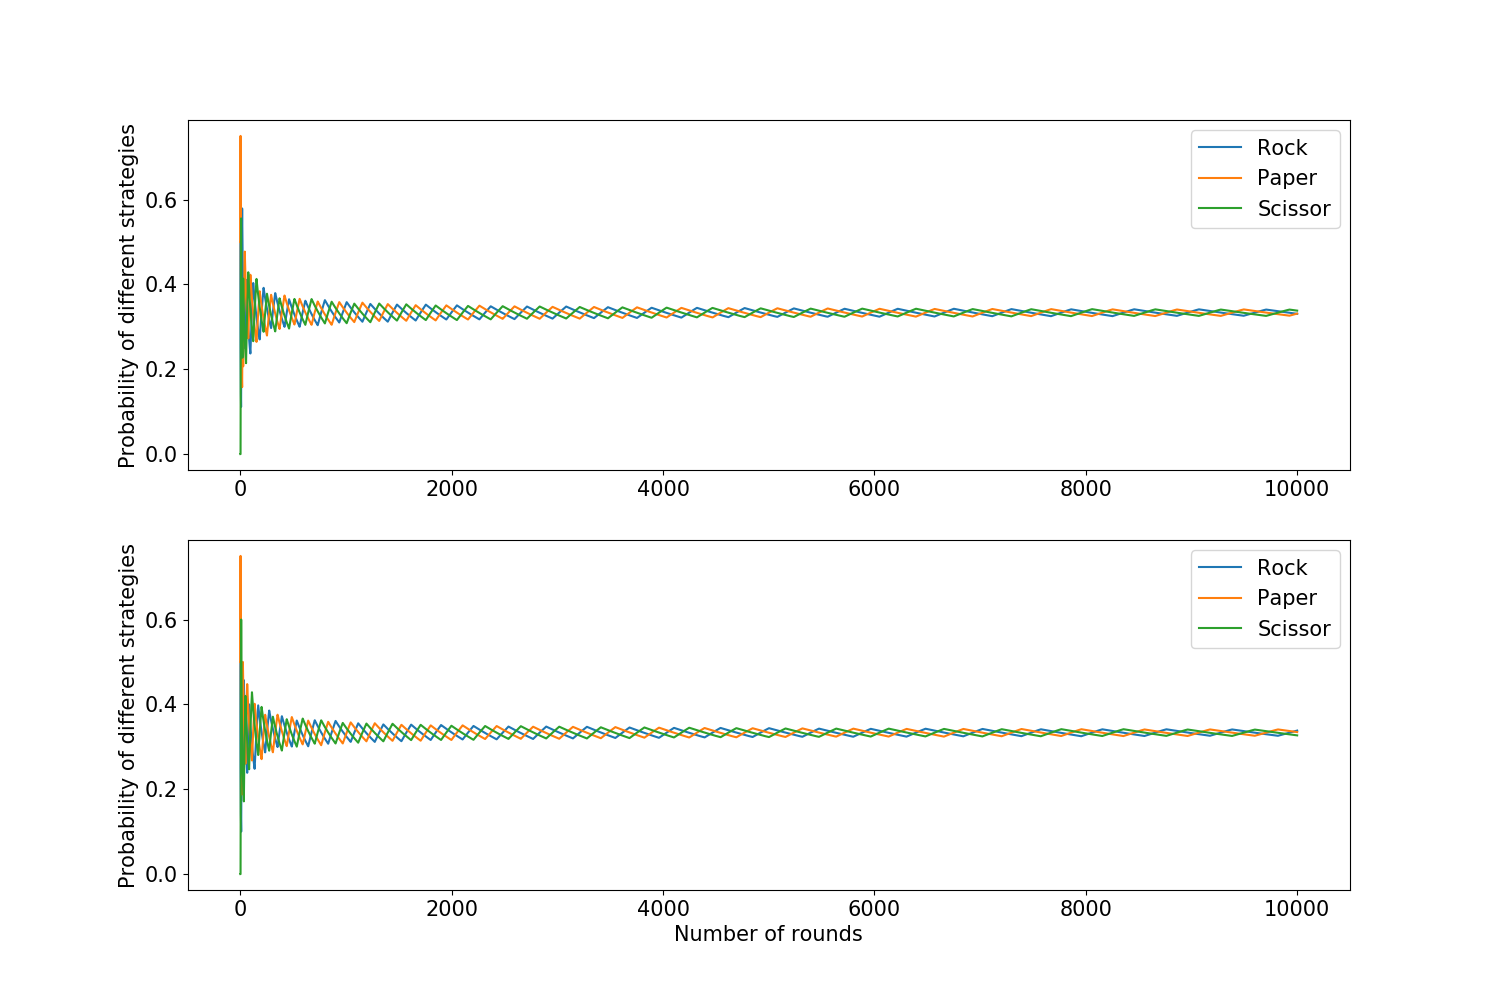
\includegraphics[width=\textwidth]{../100_100.png}
%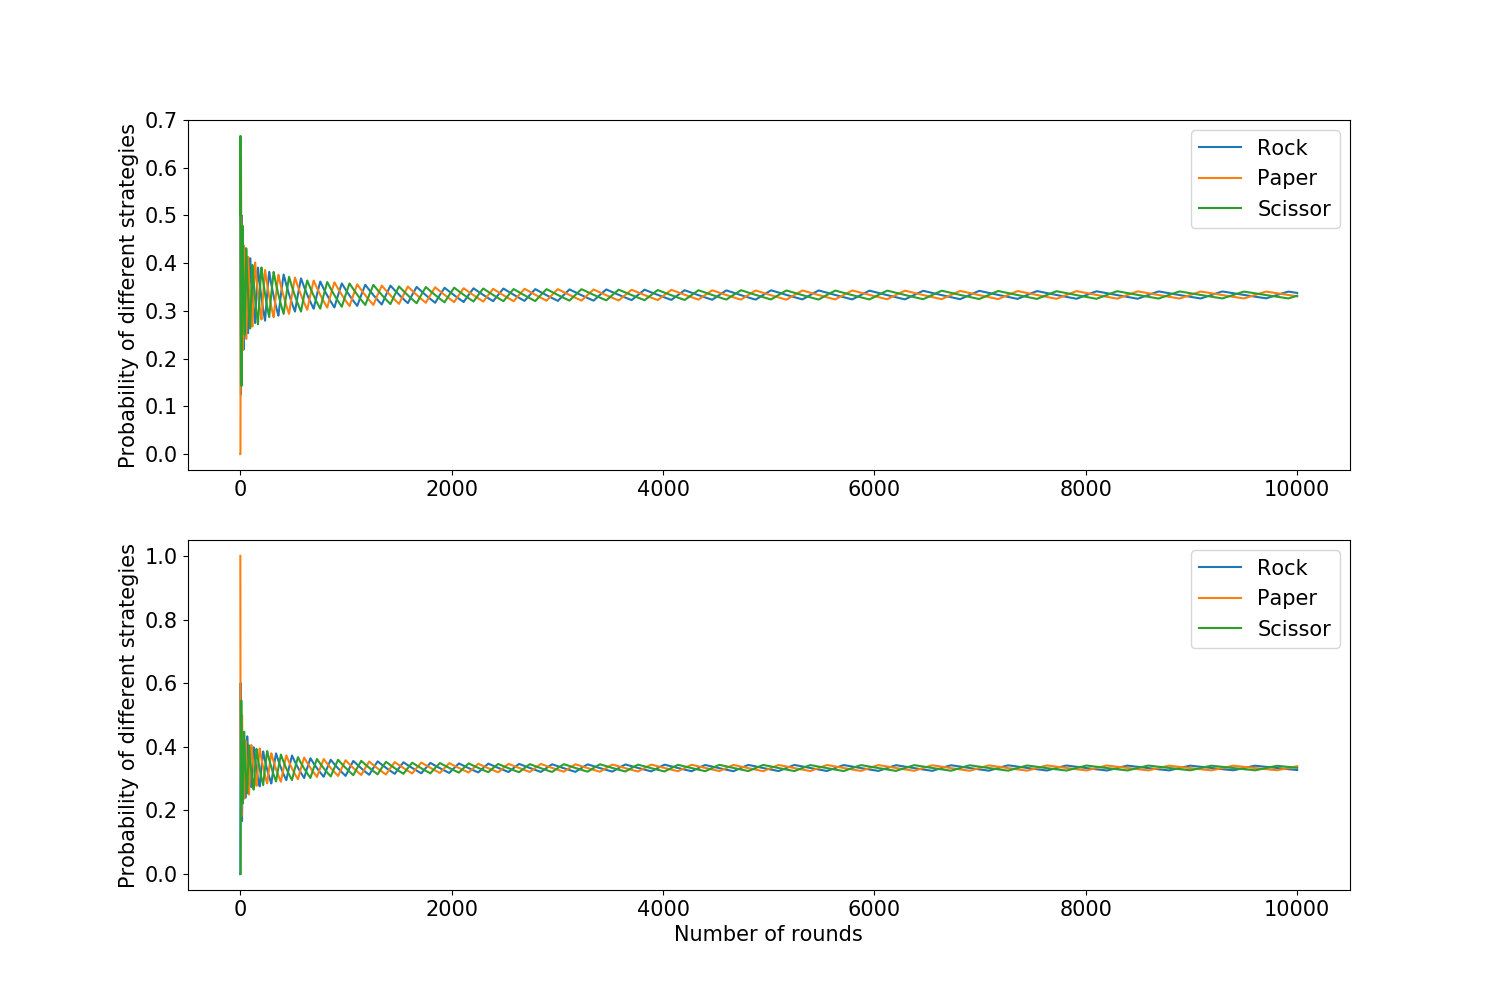
\includegraphics[width=\linewidth]{../100_010.png}
\caption{These graphs show how the \textit{statistical mixed strategies} change during the game.
We have player 1's graph on top and player 2's graph below. All the probabilities tend to converge
around 0.33, which is the only NE of the game. These graphs represent the situation in which the
first and the second player played both "rock" in the first round (similar graphs can be generated
by varying the first round).}
\end{figure}

\end{document}